\documentclass[margin,line]{res}
\usepackage[utf8]{inputenc}
\usepackage{multirow}
\usepackage{graphicx}

\oddsidemargin -.5in
\evensidemargin -.5in
\textwidth=6.0in
\itemsep=0in
\parsep=0in

\newenvironment{list1}{
  \begin{list}{\ding{113}}{%
      \setlength{\itemsep}{0in}
      \setlength{\parsep}{0in} \setlength{\parskip}{0in}
      \setlength{\topsep}{0in} \setlength{\partopsep}{0in} 
      \setlength{\leftmargin}{0.17in}}}{\end{list}}
\newenvironment{list2}{
  \begin{list}{$\bullet$}{%
      \setlength{\itemsep}{0in}
      \setlength{\parsep}{0in} \setlength{\parskip}{0in}
      \setlength{\topsep}{0in} \setlength{\partopsep}{0in} 
      \setlength{\leftmargin}{0.2in}}}{\end{list}}


\begin{document}

\name{Óscar Andrés Nájera Ocampo}

\begin{resume}

\section{\sc Información de Contacto}
  \begin{tabular}{@{}p{2in}p{2.5in}p{3cm} }
    {\it Dirección:}		& {\it casa:}  +(593-2) 241-2446 &
      \multirow{4}{*}{ 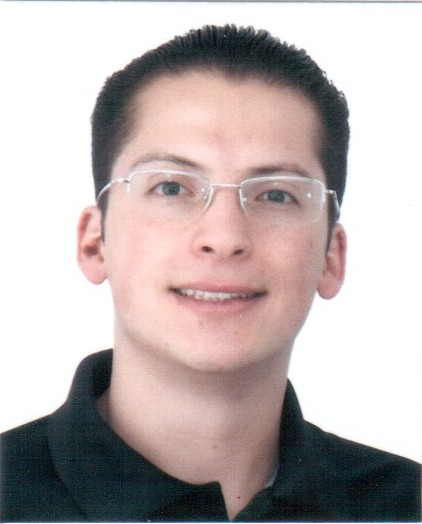
\includegraphics[width=3cm,bb=0 0 101 126]{./foto2012.jpg}}\\

    Cap. Rafael Ramos E2-254	& {\it celular:} +(593-9) 9643-9206 \\
    Casa \# 2			& {\it e-mail:}  najera.oscar@gmail.com\\
    Quito, Ecuador		& {\it www:} http://titan-c.github.com
  \end{tabular}\vspace{0.5cm}

\section{\sc Información Personal}
 \begin{tabular}{ll}
  {\it Apellidos:} Nájera Ocampo & {\it Nacimiento:} 13 April 1988\\
  {\it Nombres:} Óscar Andrés   & {\it Género:} Masculino\\
  {\it Nacionalidad:} Ecuatoriana    & %{\it Marital status:} Single
 \end{tabular}

\section{\sc Intereses investigativos}
  Materia Condensada, Física del estado sólido, Mecánica Estadística, Física Matemática y
  Teórica, Programación científica y análisis de systemas computacionales

\section{\sc Educación}
%   {\bf Universidad Central del Ecuador}, Quito, Ecuador\\
%   \vspace{-.1in}
%   \begin{list1}
%     \item[] Master in Mathematics \hfill {\bf Nov. 2012 - present}
%     \item[] Joint Master program with {\it Escuela Politécnica Nacional} \& {\it Universidad
%     San Francisco de Quito} in Quito - Ecuador and {\it Université Jean Monnet} in
%     Saint-Etienne - France
%   \end{list1}

  {\bf Escuela Politécnica Nacional}, Quito, Ecuador\\
  \vspace{-.1in}
  \begin{list1}
    \item[] Físico \hfill {\bf Oct. 2006 - Sept. 2012}\\
    \begin{list2}
    \vspace{-.1in}
      \item Tema de Tesis:  ``Estimación, por simulación computacional, la dispersión de
      la energía de interacción entre nanorregiones polares en los materiales ferroeléctricos
      relaxores $Pb_xBi_4Ti_{3+x}O_{12+3x}; x=\{2,3\}$''
      \item Director: Dr. Luis Lascano
      \item Promedio estudiantil: 8.2/10 | Tesis escrita: 9.8/10 | Defensa Oral: 10/10
    \end{list2}
  \end{list1}

  {\bf Colegio Alemán}, Quito, Ecuador\\
  \vspace{-.1in}
  \begin{list1}
    \item[] Abitur Alemán\hfill {\bf Mayo 2006}
    \item[] Bachillerato ecuatoriano \hfill {\bf Junio 2005}
  \end{list1}

\section{\sc Honores y Premios}
  Bailar por Ecuador en WDSF World DanceSport Championship Standard, Australia \hfill {\bf 2012}\\
  Primer lugar en la Olimpiada de física, Escuela Politécnica Nacional, Ecuador \hfill {\bf 2010}\\
  Medalla de Bronce por rendimiento académico, Colegio Alemán Quito, Ecuador \hfill {\bf 2005}\\
  PAD Preisträger, Kultusminister Konferenz, Alemania \hfill {\bf 2003}

\section{\sc Experiencia Académica}
  {\bf Universidad Central del Ecuador}, Quito, Ecuador
  \begin{list1}
    \item[] {\em Investigador en el grupo de Simetría molecular y química cuántica} \hfill {\bf Oct. 2012 -presente}
  \end{list1}

  {\bf Escuela Politécnica Nacional}, Quito, Ecuador
  \begin{list1}
   \item[] {\em Estudiante} \hfill {\bf Oct. 2006 - Sept. 2012}\\
    Incluye materias de carrera e investigación de tesis\\
   \item[] {\em Ayudante de laboratorio} \hfill {\bf Ago. 2011 - Junio 2012}\\
    Responsable de los laboratorios de Mecánica Newtoniana, Electromagnetismo y Óptica.\\
   \item[] {\em Auxiliar de laboratorio} \hfill {\bf Sept. 2010 - Feb. 2011}\\
    Clases de apoyo y ejercicios para los alumnos en las materias de Cálculo en una
    variable, cálculo vectorial y análisis real.
  \end{list1}

  {\bf International Center for Theoretical Physics}, Trieste, Italia
  \begin{list1}
    \item[] {\em Estudiante invitado} \hfill {\bf Feb. 20 - Mar. 2, 2012} \\
    Participación y presentación de trabajo investigativo en  {\em ``Advanced School on Scientific
    Software Development''} SMR 2330
  \end{list1}

\section{\sc Presentación en Conferencias}
  {\bf O. Nájera}, L. Lascano: ``Estimation of the exchange interaction dispersion between polar
  nano-regions in relaxors P2BIT \& P3BIT'', {\bf En:} XVI ELAVIO, {\em Latin American School in Operations Research}, Bento Gonçalves - RS - Brazil Feb. 2012.

\section{\sc Posters}
  {\bf O. Nájera}, L. Lascano: ``Estimación de la dispersión de la energía de interacción
  entre PNRs para los ferroeléctricos relaxores'',  Póster con mención de honor {\bf En:} NanoAndes, Quito-Ecuador Nov. 2012

\section{\sc Otras Publicaciones}
  {\bf O. Nájera}: ``Estimación, por simulación computacional, la dispersión de la energía de
  interacción entre nanorregiones polares en los materiales ferroeléctricos relaxores
  $Pb_xBi_4Ti_{3+x}O_{12+3x}; x=\{2,3\}$'', Tesis de grado. {\em Escuela Politécnica Nacional}, Sept. 2012.

\section{\sc Habilidades Informáticas}
  \begin{list2}
    \item Lenguajes de programación:  C/C++, Python, Bash, Php, Matlab/Octave
    \item Paquetes y librerías: GSL, SciPy, NumPy
    \item Lenguajes de descripción de contenidos: \LaTeX, HTML, CSS
    \item Sistemas Operativos: Linux(Gentoo y Ubuntu), Microsoft Windows
    \item Ofimática: LibreOffice: Writer, Calc, Impress | MsO: Word, Exel, PowerPoint
    \item Diseño gráfico: Gimp, Inkscape, Blender
  \end{list2}

\section{\sc Idiomas}
  \begin{list2}
    \item Español: Lenguaje Materno
    \item Inglés: Fluido
    \item Alemán: Fluido
  \end{list2}
  
\section{\sc Referencias personales}
 \begin{list1}
  \item[] Dr. Luis Lascano
  \begin{list2}
   \item {\it e-mail:} luis.lascano@epn.edu.ec
   \item {\it Institución:} Escuela Politécnica Nacional
   \item Director de tesis y profesor de física del estado sólido
  \end{list2}
 \end{list1}

 \begin{list1}
  \item[] Dr. Edy Ayala
  \begin{list2}
   \item {\it e-mail:} edy.ayala@epn.edu.ec
   \item {\it Institución:} Escuela Politécnica Nacional
   \item Profesor de física moderna y nuclear | Jefe del departamento de física
  \end{list2}
 \end{list1}
 
%  \begin{list1}
%   \item[] Dr. Germán Rojas
%   \begin{list2}
%    \item {\it e-mail:} german.rojas@epn.edu.ec
%    \item {\it Institution:} Escuela Politécnica Nacional
%    \item Functional Analysis teacher
%   \end{list2}
%  \end{list1}

%  \begin{list1}
%   \item[] Dr. Leonardo Basile
%   \begin{list2}
%    \item {\it e-mail:} leonardo.basile@epn.edu.ec
%    \item {\it Institution:} Escuela Politécnica Nacional
%    \item Thesis examination committee \& teacher Statistical Physics
%   \end{list2}
%  \end{list1}


\section{\sc Intereses externos}
 \begin{list2}
  \item Baile de Salón
  \item Ciclismo
  \item Natación
 \end{list2}

\end{resume}
\end{document}
